\newpage

\chapter{Evaluation of the System.}
The web application was tested and evaluated to ensure the quality of the final system. This involves using qualitative and quantitative methods to ensure the system is performing as expected. Evaluation focused on the following three key areas:

\begin{itemize}
\item Usability
\item Robustness
\item Performance
\end{itemize}

In the sections that follow we discuss how the above were tested for various levels of the system.

\section{Evaluating GUI Usability.}
One of the key requirements for the web application was to allow user to easily be able to interact with it. This involved designing a system that would be simple and clear to use. It should present the users with all the required information, abstracting them from the complexities and unnecessary details of what goes behind. Our aim was to create an application that looks and feels good, but also makes the definition of a derivation problem as clear and simple as possible.

\subsection{User testing and feedback.}
To ensure that the user experience was satisfactory we relied on user feedback to guide any design changes implemented. As the project progressed test users were given access to the graphical user interface in order to provide feedback about the design itself and additional features that might be useful. Test users included were from a wide array of backgrounds that included both people with experience in ABA frameworks, but also users that were new to ABA. This was accomplished  by relying on a group that included colleagues, friends, family and of course the supervisors of the project.

By allow the testing with users with a diverse understanding of ABA it was easier to gain feedback both on matters that technically adept users might consider important and on the general perception of the application by the public. The feedback gained was used to drive the design changes throughout the development process.

\subsection{Initial Concept.}
The project always aimed at providing a simple and understandable user interface. This implied an easy way to input a framework, configure the application and understand the output. Even though the web application is minimal and has a simple user interface, the end---product has had significant changes from the initial concept.

Initially the user interface aimed at providing the user with all the available interactions on a single page. This aimed at allowing the users to view the result, edit the framework and change the configuration all on the same page. However, this lead to an over---cluttered and confusing interface as realised from user feedback.

Additionally, various methods were considered for the input mechanism that would be implemented in order to allow the users to specify frameworks. In an attempt to make the process easier one of the ideas considered was to be able to declare rules and assumptions one---by---one using a respective for for each that asked the user for the required information (head of the rule, predicates, variable, etc). This would make it easier for users with little or no programming experience to use the application. However, user feedback showed that such an approach would be very cumbersome in terms of time. For small examples for educational purposes such an approach could potentially work, but the web application was designed in order to handle any sort of framework. As realistic ABA frameworks tend to be constructed from numerous assumptions and rules, an input mechanism had to be chosen that allowed users to easily define frameworks of any size.

Lastly, based on the feedback received from these test users additional features were added to the web applications. These are features that make the web application easier to use or provide the more technical users with exposure to the inner---working of the web application (as is the case with the grounded described in section [TODO]).

\subsection{Changes to GUI.}
Building on the feedback from out test users we proceeded to evaluate possible alternatives and implementations that would benefit them. Some of the most major contributions from the user feedback that were implemented are discussed below.

\subsubsection{Include ability to see grounded framework.}
For the more technical users access to the grounded framework can be a desirable feature. The user can look over the grounded framework and review it. This allows users to find other suitable targets they can get a derivation for and can also evaluate whether certain rules or assumptions exist as under the domain they specified.

\begin{figure}[h]
    \centering
    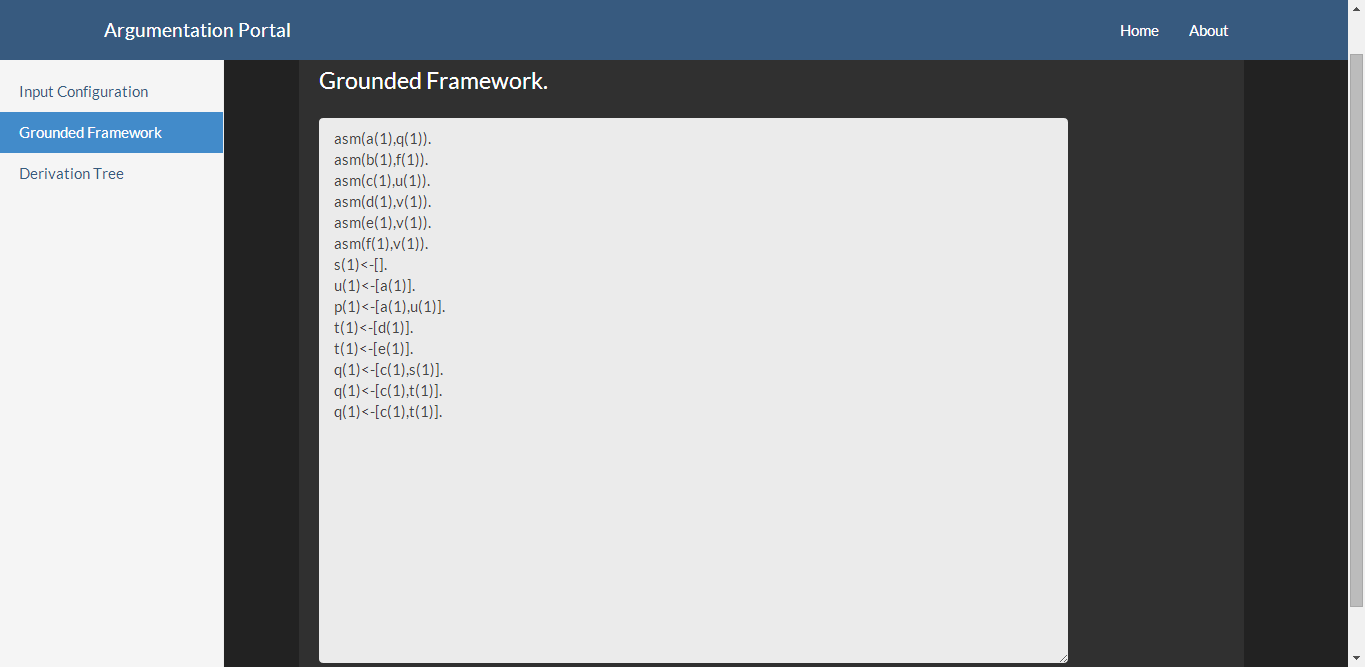
\includegraphics[width=0.8\textwidth]{argumentationGrounded.png}
    \caption{Example of the panel displaying the grounded framework.}
    \label{fig:arg_grounded}
\end{figure}

As shown in figure [TODO] the output is in a format almost identical to the format the user used ton define the framework in the first place. Additionally, when grounding a framework over an extensive domain it is expected that there might be a significant increase in the number of rule and assumption definitions. Therefore, the window provided is both scrollable and resizeable. Furthermore it is also read---only to avoid any tampering with the grounded framework.

\subsubsection{Tabulated sections.}
Following from the feedback gathered that described the initial interface as over---cluttered and confusion, we separated the sections in easily reachable and distinct panels that each serves a specific purpose. The section are:

\begin{itemize}
\item Input Configuraion.
\item Grounded Framework.
\item Derivation Tree.
\end{itemize}

All the tabs exist in the same session and switching between tabs is handled client---side by selecting the appropriate section from the navigation panel on the left as shown in image [TODO]. This allows for easy and simple navigation between the various aspects of the web application. It also provides the users with ability to change the input framework and the configurations on the fly.

\begin{figure}[h]
    \centering
    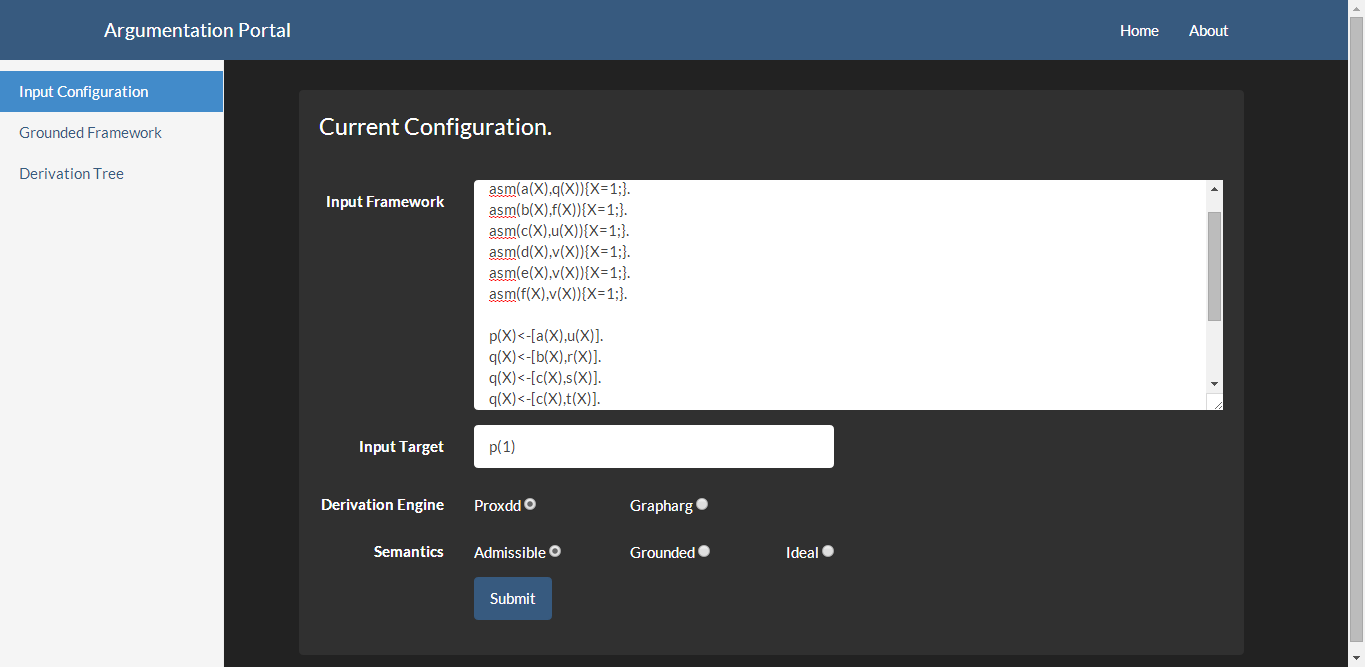
\includegraphics[width=0.8\textwidth]{argumentationInputFull.png}
    \caption{The input configuration tab.}
    \label{fig:arg_input_tab}
\end{figure}

\begin{figure}[h]
    \centering
    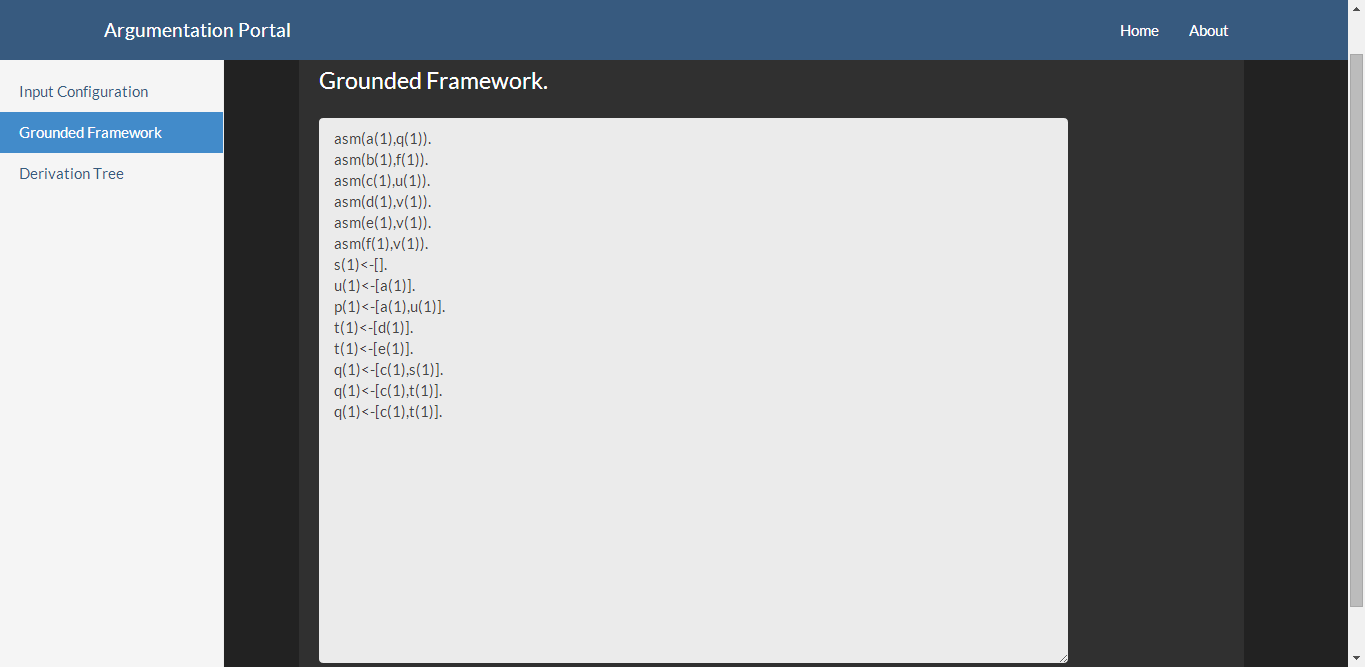
\includegraphics[width=0.8\textwidth]{argumentationGrounded.png}
    \caption{The grounded framework tab.}
    \label{fig:arg_grounded_tab}
\end{figure}

\begin{figure}[h]
    \centering
    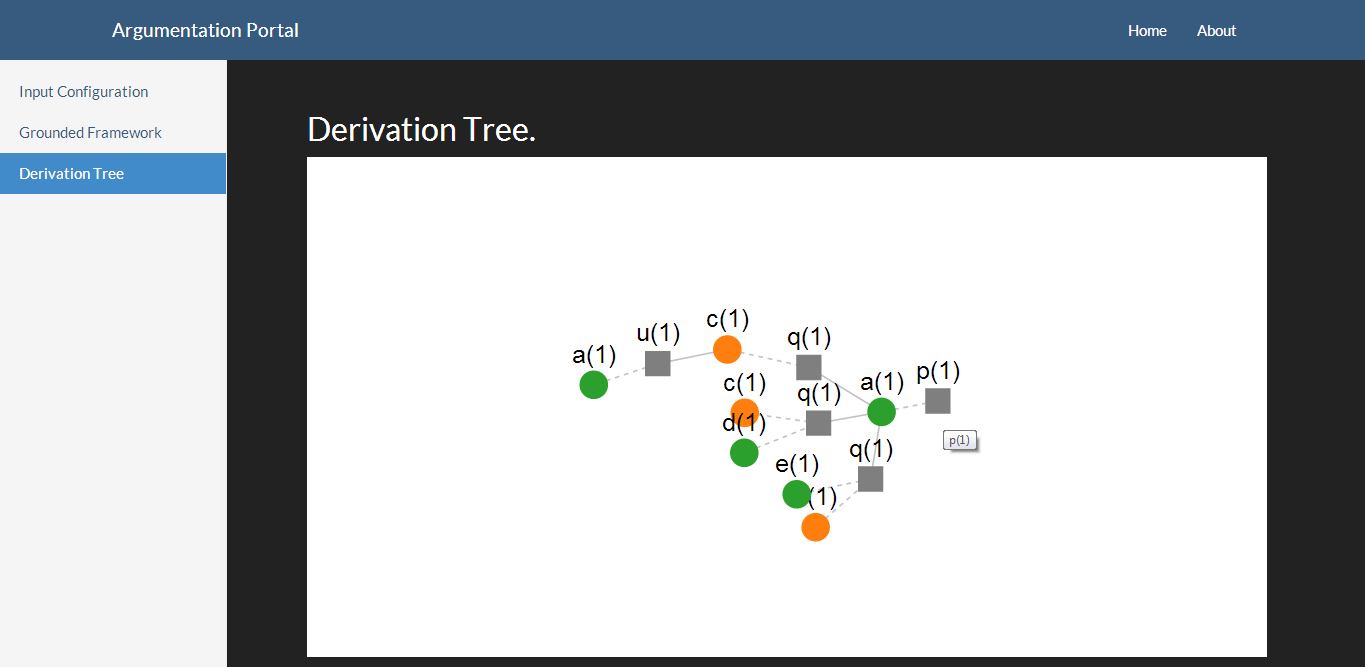
\includegraphics[width=0.8\textwidth]{argumentationTree.png}
    \caption{The derivation tree tab.}
    \label{fig:arg_tree_tab}
\end{figure}

\subsubsection{Bootstrap based GUI.}
Lastly, the general design and colour scheme used for the web application was deemed uncreative and dull. Therefore, to ensure a better user experience and to instill faith in the system's capabilities the user interface was re---designed to a more polished---up look. This was done using a popular tool that allows for the creation of good looking web application and websites called Bootstrap. Although the underlying functionalities of the web application are exactly the same, the final looked received better feedback from users, who now seemed more confident using the systems. The difference can be seen in figures [TODO] and [TODO].

[TODO] - Add image of before.

[TODO] - Add image of after.

\section{Evaluating the Grounder.}
Ensuring the validity of the grounder is important in ensuring the validity of the whole system. As a preprocessing step, if this is not carried out correctly then we risk passing to the derivation engine wrong or even invalid input. Therefore, we need to ensure the robustness of our grounding mechanism with both large and small frameworks. Specifically during the evaluation process for the grounder we seeked to verify the following:

\begin{itemize}
\item Correct Grounding of frameworks over their domain.
\item Robustness when dealing with large scale frameworks.
\item Satisfying performance for our grounder.
\end{itemize}

\subsection{Checking validity through examples.}
Initially we tested the grounder by running the examples we used to test the derivation engines in general, adapted however to include domains. This means that the example frameworks now have to be grounded first before they get provided to the derivation engine. By isolating the grounded we were able to provide the input for which we knew the expected output and then compare this to the actual output received. 

There are three cases which we needed to check how they were grounded. These represent the three valid forms of the commands we can provide based on the language we have defined. These are:

\begin{itemize}
\item \emph{asm(a(X),b(X))} - This defines an assumption that exists on the domain specified by the user.
\item \emph{a(X)\textless-[]} - This defines a fact. A fact is handled by the grounder similarly to assumptions.
\item \emph{a(X)\textless-[b(X)]} - This defines a rule which can exist if the predicates in the detail exist in the global domain of our framework.
\end{itemize}

The examples we used had to accommodate and test all of these cases. Consider example [TODO] which is one of the examples used.

\begin{Verbatim}[frame=single]
b(X,A)<-[a(X,A)].
asm(a(X,Y),d(Y)){X=1,2;Y=2,3;}.
c(X,Y,Z)<-[]{X=1,3;Y=2,3;Z=Michael,John;}.
\end{Verbatim}

\begin{Verbatim}[frame=single]
asm(a(1,2),d(2)).
asm(a(2,2),d(2)).
asm(a(1,3),d(3)).
asm(a(2,3),d(3)).
c(1,2,Michael)<-[].
c(3,2,Michael)<-[].
c(1,3,Michael)<-[].
c(3,3,Michael)<-[].
c(1,2,John)<-[].
c(3,2,John)<-[].
c(1,3,John)<-[].
c(3,3,John)<-[].
b(2,3)<-[a(2,3)].
b(1,3)<-[a(1,3)].
b(2,2)<-[a(2,2)].
b(1,2)<-[a(1,2)].
\end{Verbatim}

This way we ensured that the grounding was carried out successfully. 

\subsection{Random Framework generator.}
Later on in our evaluation of the grounder we explored the possibility of test running the grounder using large random frameworks. This would enable us to both check the validity of the grounder, but also to test its performance against frameworks of a larger scale.

\subsubsection{How the random generator works.}

However, creating such frameworks by hand is cumbersome and prone to errors. Therefore, we devised an algorithm for pseudo---random framework generations which is described in [TODO].

[TODO] - Pseudo code for random framework generation.
\begin{Verbatim}[frame=single]
Procedure genRandFramework()
	int[] domainA
	int[] domainB
	Dictionary assumCont
	Queue assumQ
	Queue ruleQ
	List framework
	List frameworkAssums
	List frameworkRules
	List startSymbols = getStartList()
	List availableSymbols = startSymbols
	
	ruleQ.Enqueue("a")
	
	while( (assumQ and ruleQ not empty) 
			and availableSymbols not empty)
		if(assumQ not empty)
			assum = createAsm(assumQ.Dequeue,
				startSymbols,assumCont)
			frameworkAssums.Add(assum)
		else
			rule = createRule(ruleQ.Dequeue,
				availableSymbols,assumQ,ruleQ)
			frameworkRules.Add(rule)
			
	foreach assumption in frameworkAssums
		framework.Add(assumption)
	
	foreach rule in frameworkRules
		framework.Add(rule)
end
		
Procedure createAsm(id,startSymbols,assumCont)
	/* Pick Random Contrary from startSymbols */
	/* Randomly choose between possible domains */
	/* Add assumption and contrary pair to Dictionary */
	/* Construct assumption and return */
end

Procedure createRules(id,availableSymbols,assumQ,ruleQ)
	/* Randomly choose number of terms in rule's */
	/* tail (between 1-4) */
	/* Randomly pick terms's Ids from availableSymbols */
	/* and remove from availableSymbols */
	/* Randomly add each of the tail terms to either */
	/* assumQ or ruleQ */
	/* Construct Rule and return */
end

\end{Verbatim}

\subsubsection{Grounding large scale frameworks.}

Having implemented this algorithm we were now able to create random frameworks and check whether they were grounded correctly. Additionally we used the generation of large frameworks to test the performance.

Example [TODO] shows an example of the ungrounded framework and example [TODO] show the respective grounded framework. As the large scale frameworks would be hard to provide as part of this report, we take a smaller framework to be indicative of the process carried out with the larger frameworks as well. In these examples we consider a frameworks made up of approximately 20-30 commands.[TODO] check.

[TODO] - add ungroundedn and grounded


\subsection{Performance of Grounder.}

[TODO] - Performance analysis.

As explained in section [TODO] there are optimisation mechanism that can be implemented to improve the performance

\section{Evaluating the ideal semantics implementation.}
During the implementation of the project I also got the opportunity to work with the derivation engines directly. The aim was to extend the Proxdd derivation engine to be able to accommodate derivations based on ideal semantics as described in section [TODO].

In order to be able to add the extended derivation engine to the web application we first had to ensure that the required functionality was carried out properly. In order to do so the semantics had to be tested with several example of which we had an expected outcome.

Due to the nature of definition of the ideal semantics derivation (as described in section [TODO]) we were able to implement it in two stages. This also made the testing process easier. The evaluation of the validity of our ideal semantics derivation  was broken down in the following steps:

\begin{enumerate}
\item Ensure the correct updating of the F set.
\item Test the cases for the Fail(S) derivations.
\item Test the complete implementation with examples.
\end{enumerate}

\subsection{Testing in Swi---Prolog.}
The design of the web application is such by which changes in the derivation engines can be carried out without affecting the rest of the application. Therefore, our implementation of the ideal semantics could easily be tested directly in Swi-Prolog through its console to ensure its validity and only add it to the existing project one we were sure it was safe.

This approach provides us with various advantages:

\begin{itemize}
\item Ability to debug using Swi-Prolog debugging tools.
\item Ability to test the predicates that make up the derivation individually.
\item Ability to easily test using predefined examples defined in files.
\end{itemize}

Since the application is unaffected by the required changes to implement the ideal semantics, we were able to carry out the testing using the Swi-Prolog console. We the simply integrated the derivation engine including the ideal semantics in the existing web application.

\subsubsection{Testing updating of F set.}
The first step in implementing the ideal semantics is establishing and updating correctly the F-Set as described in section [TODO]. This requires extending the existing admissible derivation, but does not require changes that will alter the functionality of the admissible based derivations. Therefore, we can implement the F set as an extension of the admissible based derivation and check that it is updated correctly during an admissible derivation.

As defined in algorithm [TODO] the F set is updated  depending on the turn and case we are facing at that part of the derivation, just like the other sets in the tuple are. Additionally, the algorithm itself is turn based. At every turn the tuple is updated accordingly and the whole process is repeated again until certain conditions apply. Therefore, we decided to check that at every possible case in every possible turn the updating of the F-set is done correctly.

This is done by using the Swi-Prolog console to test the updating of the tuple at every possible case of the derivation algorithm individually. This is done by providing a tuple as an input for which we are aware of the expected output. Constructing such examples was simple as the logic used to update the  set was primitive. Therefore, constructing such test tuples and finding their outputs was easily done by hand. Consider example [TODO]. 

[TODO] - Add example of a single step check.

By testing all of the checks individually we can ensure that the updating is carried out successfully at each case. This also makes it easier to detect and correct bugs relating to the updating. Once the updating has been verified then the rest should still be valid because it has already been implemented as part of the admissible derivations. The whole implementation so far was lastly tested by running full examples under admissible semantics and observing and verifying the updating of the F set during said derivations, as in example [TODO].

[TODO] - ADD FULL EXAMPLE

\subsubsection{Testing Fail(S) derivations.}
The approach described in the section above was similarly used to test the implementation of the Fail(S) derivations used in the ideal based derivations. The algorithm described in section [TODO] that carries out the Fail(S) derivation, involves the generation of tuples from other tuples in a turn based manner. 

By implementing the algorithm as a series of predicates rather than just one large predicate we were able to test the validity of each predicate individually. This again implied providing a predefined tuple as an input and comparing the output to the expected output we derived by hand, as shown in example [TODO]

[TODO] - Add example.

Similarly before we integrate the fail derivation in the system we ensured that as a whole it worked correctly by trying out examples we could work through the derivation by hand. We then provided the starting tuple to the fail derivation predicate and verified that the derivation was carried out correctly, as in example [TODO].

[TODO] - Example.

Fail(S) derivations by definition either succeed or fail, which makes it hard to understand whether the derivation was carried out correctly or not. In order to verify this we run the predicate carrying out the derivation in the Swi-Prolog console while having set the \emph{guitracer} mode on and having set relevant spy points. This allowed us to verify that at each turn of the derivation the expected tuples were being created and that we did not just end up with the desired outcome by luck.

\subsubsection{Testing the ideal based derivations as a whole.}
Having ensured the validity of the individual parts that allow us to run derivations under ideal semantics and having integrated them in the current derivation engine, we now had to ensure that the ideal based derivations worked as expected from start to finish. In order to verify this we used frameworks that were designed to verify that the derivation responds as it should. These could be considered as test cases that ensured that the ideal based derivations were correct.

This examples were designed with the theory behind ideal semantics in mind and ensured to test various cases for which ideal derivations should or should not exist.

[TODO] - BIG CHUNK. ADD Toni examples and explain the case of each.